%--------------------------------- Timing Constraints (DCC+TVA) - Preface -----------------------------------------------
% (9)
\subsubsection{Timing Constraints considering DCC and Technology Leader}
\label{sec:TVA:timingconstraint}
\begin{figure*}
    \centering
    \subfigure[Case 2-1: One leader on the common clock path (e.g., at buffer 1), and two DCCs]{
    	\label{fig:sub:dccleaderi1}
        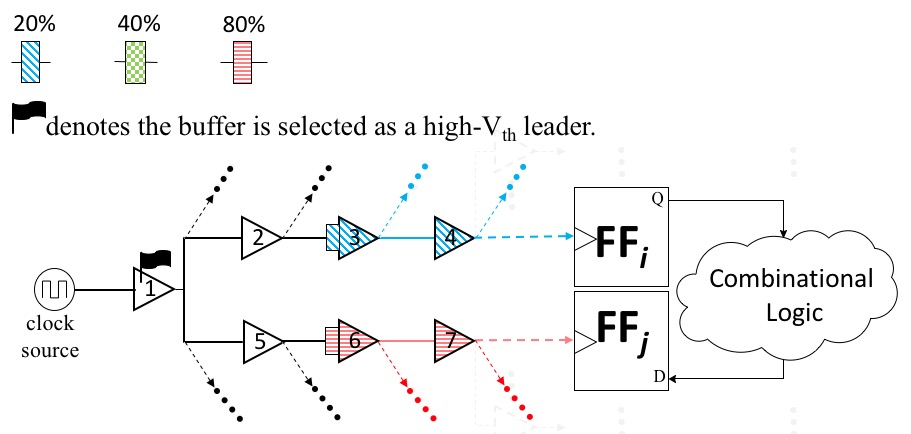
\includegraphics[width=0.9\columnwidth]{2DCC_1Leader.png}
    }
    \hspace{1cm}
    \subfigure[Case 2-2: one leader on one of the divergent clock paths, or class 3: two leaders, one on each of the divergent clock paths]{
    	\label{fig:sub:dccleaderi2}
        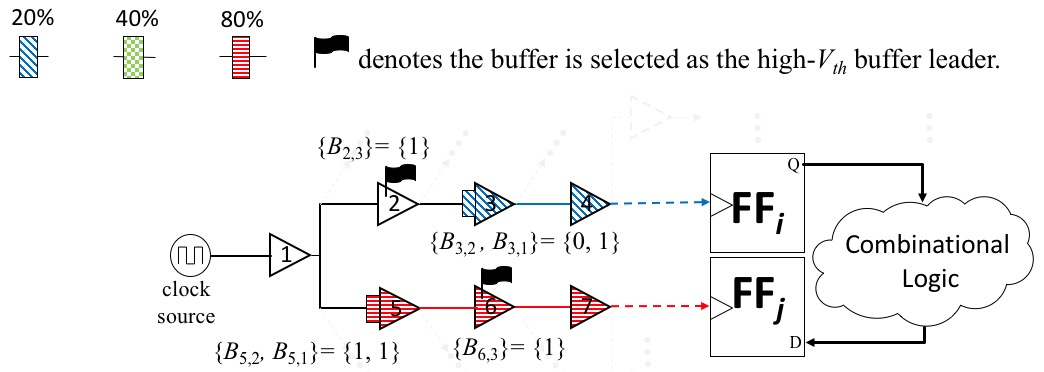
\includegraphics[width=0.9\columnwidth]{2DCC_2Leader.png}
    }
    \caption{Examples of DCC insertion}
    \label{fig:dccleaderinsert}
\end{figure*}
The timing constraints, considering the two techniques, is extended from those in Section~\ref{subsec:tccc}. As seen in Section~\ref{subsec:tccc}, given a pair of flip-flops, between which there exists one logic path, the timing (i.e., setup-time and hold-time) constraints must be met based on the inequalities Equation~(\ref{eq:tsu}) and~(\ref{eq:th}). The former timing constraints in Section~\ref{subsec:tccc} only consider the impact of DCC deployment on clock latency. Thus, the new timing constraints here must consider the impact of V\textsubscript{th} assignment on clock latency. 

Given one clock period $T_c$ derived by binary search, one aging-critical logic path, and its associated clock network, the former timing constraints are classified into 3 classes, according to the used DCC count (i.e., no, one, and two DCC insertions). The new timing constraints are extended from the 3 classes, each of which are further classified into 3 subclasses, according to the leader count (i.e., the count of buffers which are selected as leaders). Thus, there are totally 9 (= $3*3$) subclasses based on the count of DCC and leader. For brevity, 6 of the 9 subclasses are omitted in the following discussion. We only discuss the other 3 subclasses, whose DCC deployments are identical, but leader counts vary from 0, 1 to 2. Furthermore, due to the aforementioned DCC and leader constraints, the SAT solver will only output a DCC (leader) deployment (selection) where there does not exist more than one DCC (leader) along any clock path. Thus, in the following discussion, the deployment (selection) with more than one DCC (leader) along a single clock path can be ignored. In each subclass, if the DCC (leader) deployment (selection) causes a timing violation within 10 years (i.e., the lifespan specification), then the deployment (selection) will be transformed into CNF clauses, such that the solver will not output the deployment (selection) as results. Here, we explain the generation of CNF clauses by using the example in Figure~\ref{fig:dccleaderinsert}.

%--------------------------------- Timing Constraints (DCC+TVA) - Class 1 -----------------------------------------------
\setcounter{class}{0}
\begin{class}
\label{class:c4}
No buffer on either clock path is selected as a technology leader

Consider the situation that, among buffers 1 $\hyphen$ 7, no buffer is selected as a technology leader. If it causes a timing violation along the aging-critical path within 10 years, then the Boolean representation of the deployment,{\fontsize{8}{8.4}
\begin{gather*}
\left(\{B_{1,3}, B_{1,2}, B_{1,1}\} \equiv \{0, 0, 0\} \right) 
\land \left( \{B_{2,3}, B_{2,2}, B_{2,1}\} \equiv \{0, 0, 0\} \right) \\ \land \dotsb 
\land \left( \{B_{7,3}, B_{7,2}, B_{7,1}\} \equiv \{0, 0, 0\} \right),
\end{gather*}}
equivalent to the following CNF clause:
{\fontsize{8}{8.4}$(B_{1,3} \lor B_{1,2} \lor B_{1,1} \lor B_{2,3} \lor B_{2,2} \lor B_{2,1} \lor \dotsb \lor B_{7,2} \lor B_{7,2} \lor B_{7,1} )$,}
should be generated such that the solver will not output the corresponding DCC deployment and leader selection in the result if the CNF is satisfiable. In this case, a total of 1 CNF clause is generated.
\end{class}

%--------------------------------- Timing Constraints (DCC+TVA) - Class 2 -----------------------------------------------
\begin{class}
\label{class:c5}
Only one buffer is selected as a technology leader

This class can be further classified into 2 sub-classes based on the buffer location of technology leader. \\
\textit{Class 2-1:} Selected buffer (i.e., technology leader) on the common clock path.

In Figure~\ref{fig:dccleaderinsert}, buffer 1 is on the common clock path. Consider the leader selection shown in Figure~\ref{fig:sub:dccleaderi1}: if buffer 1 is the high-V\textsubscript{th} leader and the leader selection causes a timing violation within 10 years, then the Boolean representation of the technology leader selection and the DCC deployment, 
{\fontsize{8}{8.4}
\begin{gather*}
\left(\{B_{1,3}, B_{1,2}, B_{1,1}\} \equiv \{1, 0, 0\} \right) \land \left( \{B_{2,3}, B_{2,2}, B_{2,1}\} \equiv \{0, 0, 0\} \right) \\ \land \left( \{B_{3,3}, B_{3,2}, B_{2,1}\} \equiv \{0, 1, 0\} \right) \land \left( \{B_{4,3}, B_{4,2}, B_{4,1}\} \equiv \{0, 0, 0\} \right) \\ \land \left( \{B_{5,3}, B_{5,2}, B_{5,1}\} \equiv \{0, 0, 0\} \right) \land  \left( \{B_{6,3}, B_{6,2}, B_{6,1}\} \equiv \{0, 1, 1\} \right) \\ \land \left( \{B_{7,3}, B_{7,2}, B_{7,1}\} \equiv \{0, 0, 0\} \right),
\end{gather*}
}
equivalent to the following clause: 
{\fontsize{8}{8.4}$(\neg B_{1,3} \lor B_{1,2} \lor B_{1,1} \lor B_{2,3} \lor B_{2,2} \lor B_{2,1} \lor B_{3,3} \lor \neg B_{3,2} \lor B_{3,1} 
\lor B_{4,3} \lor B_{4,2} \lor B_{4,1} \lor B_{5,3} \lor B_{5,2} \lor B_{5,1} \lor B_{6,3} \lor \neg B_{6,2} \lor B_{6,1}  
\lor B_{7,3} \lor B_{7,2} \lor B_{7,1} )$}, should be generated such that the solver will not output the leader selection and DCC deployment in the result if the CNF is satisfiable. Given that there are 1 choices of technology leader, a total of 1 CNF clause will be generated in the worst case.

%DATE 2018
%if the insertion of a 40\% DCC at buffer 1 causes a timing violation within 10 years, then the Boolean representation of the DCC deployment, $\left(\{B_{1,2}, B_{1,1}\} \equiv \{1, 0\} \right) \land \left( \{B_{2,2}, B_{2,1}\} \equiv \{0, 0\} \right) \land \dotsb \land \left( \{B_{7,2}, B_{7,1}\} \equiv \{0, 0\} \right)$, equivalent to the following clause: $\left(\neg B_{1,2} \lor B_{1,1} \lor B_{2,2} \lor B_{2,1} \lor \dotsb \lor B_{7,2} \lor B_{7,1} \right)$, should be generated such that the solver will not output the deployment in the result if the CNF is satisfiable. Given that there are 3 choices of DCCs, a total of 3 CNF clauses will be generated in the worst case. \\

%\textit{Class 2-2:} \mbox{\fontsize{9}{10.8}\selectfont Selected buffer (i.e., technology leader) is on one of the divergent clock paths}
\textit{Class 2-2:} Selected buffer (i.e., technology leader) is on one of the divergent clock paths.

This class targets buffers 2, 3, 4, 5, 6, 7. If buffer 2 is the high-V\textsubscript{th} leader, and it causes a timing violation within 10 years, then the Boolean representation of the leader selection and the DCC deployment, 
{\fontsize{8}{8.4}
\begin{gather*}
\left(\{B_{2,3}, B_{2,2}, B_{2,1}\} \equiv \{1, 0, 0\} \right) \land \left( \{B_{1,3}, B_{1,2}, B_{1,1}\} \equiv \{0, 0, 0\} \right) \\ 
\land \left( \{B_{3,3}, B_{3,2}, B_{3,1}\} \equiv \{0, 1, 0\} \right) \land \left( \{B_{4,3}, B_{4,2}, B_{4,1}\} \equiv \{0, 0, 0\} \right) \\ 
\land \left( \{B_{5,3}, B_{5,2}, B_{5,1}\} \equiv \{0, 0, 0\} \right) \land \left( \{B_{6,3}, B_{6,2}, B_{6,1}\} \equiv \{0, 1, 1\} \right) \\ 
\land \left( \{B_{7,3}, B_{7,2}, B_{7,1}\} \equiv \{0, 0, 0\} \right),
\end{gather*}
}
equivalent to the following CNF clause: 
{\fontsize{8}{8.4}$(B_{1,3} \lor B_{1,2} \lor B_{1,1} \lor \neg B_{2,3} \lor B_{2,2} \lor B_{2,1} \lor B_{3,3} \lor \neg B_{3,2} \lor B_{3,1} \lor B_{4,3} \lor B_{4,2} \lor B_{4,1} \lor B_{5,3} 
\lor B_{5,2} \lor B_{5,1} \lor B_{6,3} \lor \neg B_{6,2} \lor  \neg B_{6,1} \lor B_{7,3} \lor B_{7,2} \lor B_{7,1} )$}, should be generated such that the solver will not output the leader selection and DCC deployment in the result if the CNF is satisfiable. This class includes 6 candidates: buffers 2, 3, 4, 5, 6, 7, and each has 1 choice of technology leader. Therefore, a total of 6 CNF clauses will be generated in the worst case.
%DATE 2018
%This class targets buffers 2, 3, 4, 5, 6, 7. If the insertion of a 20\% DCC at buffer 3 causes a timing violation within 10 years, then the Boolean representation of the DCC deployment, $\left(\{B_{3,2}, B_{3,1}\} \equiv \{0, 1\} \right) \land \left( \{B_{1,2}, B_{1,1}\} \equiv \{0, 0\} \right) \land \dotsb \land \left( \{B_{7,2}, B_{7,1}\} \equiv \{0, 0\} \right)$, equivalent to the following CNF clause: $\left(B_{3,2} \lor \neg B_{3,1} \lor B_{1,2} \lor B_{1,1} \lor B_{2,2} \lor B_{2,1} \lor \dotsb \lor B_{7,2} \lor B_{7,1} \right)$, should be generated such that the solver will not output the deployment in the result if the CNF is satisfiable. This class includes 6 candidates: buffers 2, 3, 4, 5, 6, 7, and each has 3 choices of DCCs. Therefore, a total of 18 CNF clauses will be generated in the worst case.
\end{class}
%--------------------------------- Timing Constraints (DCC+TVA) - Class 3 -----------------------------------------------
\begin{class}
\label{class:c6}
Two buffers on two divergent clock paths are selected as technology leaders.

Given the DCC deployment and leader selection in Figure~\ref{fig:sub:dccleaderi2} (a 20\% DCC inserted at buffer 3, a 80\% DCC inserted at buffer 6, and buffer 2 and 5 are both  high-V\textsubscript{th} leaders), if it causes a timing violation along the aging-critical path within 10 years, then the Boolean representation of the deployment, 
{\fontsize{8}{8.4}
\begin{gather*}
\left(\{B_{1,3}, B_{1,2}, B_{1,1}\} \equiv \{0, 0, 0\} \right) \land \left( \{B_{2,3}, B_{2,2}, B_{2,1}\} \equiv \{1, 0, 0\} \right) \\ 
\land \left( \{B_{3,3}, B_{3,2}, B_{3,1}\} \equiv \{0, 1, 0\} \right) \land \left( \{B_{4,3}, B_{4,2}, B_{4,1}\} \equiv \{0, 0, 0\} \right) \\ 
\land \left( \{B_{5,3}, B_{5,2}, B_{5,1}\} \equiv \{1, 0, 0\} \right) \land \left( \{B_{6,3}, B_{6,2}, B_{6,1}\} \equiv \{0, 1, 1\} \right) \\ 
\land \left( \{B_{7,3}, B_{7,2}, B_{7,1}\} \equiv \{0, 0, 0\} \right),
\end{gather*}
}
equivalent to the following  CNF clause: 
{\fontsize{8}{8.4}$(B_{1,3} \lor B_{1,2} \lor B_{1,1} \lor \neg B_{2,3} \lor B_{2,2} \lor B_{2,1} \lor B_{3,3} \lor \neg B_{3,2} \lor B_{3,1} \lor B_{4,3} \lor B_{4,2} \lor B_{4,1} \lor \neg B_{5,3} \\
\lor B_{5,2} \lor B_{5,1} \lor B_{6,3} \lor \neg B_{6,2} \lor  \neg B_{6,1} \lor B_{7,3} \lor B_{7,2} \lor B_{7,1} )$}, should be generated such that the solver will not output the deployment in the result if the CNF is satisfiable.

Class 3 considers the selection of the two technology leaders, one among buffers \{2, 3, 4\} and the other one among buffers \{5, 6, 7\}; thus, there are totally 9 (=$3^2$) possibilities of high-V\textsubscript{th} leader selection. Therefore, a total of 9 CNF clauses will be generated in the worst case.

Considering all of the above cases with the given DCC deployment, a maximum number of 1 + 1 + 6 + 9 = 17 clauses can be derived. This is based on the existence of 12 clauses introduced in Section~\ref{sec:TVA:dcc_c}. If we consider the 103 possibilities of DCC deployment in Section~\ref{subsec:tccc}, a total of 1751 (=$103*17$) clauses can be derived in the worst case.

\end{class}
